\documentclass[tikz,border=10pt]{standalone}
% Shared look for every TikZ diagram. Load with % Shared look for every TikZ diagram. Load with % Shared look for every TikZ diagram. Load with \input{../../tools/tikz-style.tex}
\usepackage[T1]{fontenc}
\usepackage{lmodern}
\renewcommand{\sfdefault}{lmr}  % diagrams use the same serif as the text
\usetikzlibrary{arrows.meta, positioning, shapes.geometric, calc, fit, backgrounds}
\definecolor{cblue}{HTML}{4C78A8}
\definecolor{corange}{HTML}{F58518}
\definecolor{cgreen}{HTML}{54A24B}
\definecolor{cred}{HTML}{E45756}
\definecolor{cpurple}{HTML}{B279A2}
\definecolor{cgrey}{HTML}{6B6B6B}
\tikzset{
  every picture/.style={font=\sffamily, line width=1.2pt},
  box/.style={draw=#1, fill=#1!12, rounded corners=4pt, align=center, inner sep=7pt, minimum height=1.1cm},
  box/.default=cgrey,
  arrow/.style={-{Stealth[length=3mm]}, draw=cgrey, line width=1.4pt},
  title/.style={font=\sffamily\bfseries\Large},
  note/.style={font=\sffamily\small, text=cgrey, align=center},
}
\AtBeginDocument{\hyphenpenalty=10000 \exhyphenpenalty=10000}

\usepackage[T1]{fontenc}
\usepackage{lmodern}
\renewcommand{\sfdefault}{lmr}  % diagrams use the same serif as the text
\usetikzlibrary{arrows.meta, positioning, shapes.geometric, calc, fit, backgrounds}
\definecolor{cblue}{HTML}{4C78A8}
\definecolor{corange}{HTML}{F58518}
\definecolor{cgreen}{HTML}{54A24B}
\definecolor{cred}{HTML}{E45756}
\definecolor{cpurple}{HTML}{B279A2}
\definecolor{cgrey}{HTML}{6B6B6B}
\tikzset{
  every picture/.style={font=\sffamily, line width=1.2pt},
  box/.style={draw=#1, fill=#1!12, rounded corners=4pt, align=center, inner sep=7pt, minimum height=1.1cm},
  box/.default=cgrey,
  arrow/.style={-{Stealth[length=3mm]}, draw=cgrey, line width=1.4pt},
  title/.style={font=\sffamily\bfseries\Large},
  note/.style={font=\sffamily\small, text=cgrey, align=center},
}
\AtBeginDocument{\hyphenpenalty=10000 \exhyphenpenalty=10000}

\usepackage[T1]{fontenc}
\usepackage{lmodern}
\renewcommand{\sfdefault}{lmr}  % diagrams use the same serif as the text
\usetikzlibrary{arrows.meta, positioning, shapes.geometric, calc, fit, backgrounds}
\definecolor{cblue}{HTML}{4C78A8}
\definecolor{corange}{HTML}{F58518}
\definecolor{cgreen}{HTML}{54A24B}
\definecolor{cred}{HTML}{E45756}
\definecolor{cpurple}{HTML}{B279A2}
\definecolor{cgrey}{HTML}{6B6B6B}
\tikzset{
  every picture/.style={font=\sffamily, line width=1.2pt},
  box/.style={draw=#1, fill=#1!12, rounded corners=4pt, align=center, inner sep=7pt, minimum height=1.1cm},
  box/.default=cgrey,
  arrow/.style={-{Stealth[length=3mm]}, draw=cgrey, line width=1.4pt},
  title/.style={font=\sffamily\bfseries\Large},
  note/.style={font=\sffamily\small, text=cgrey, align=center},
}
\AtBeginDocument{\hyphenpenalty=10000 \exhyphenpenalty=10000}

\begin{document}
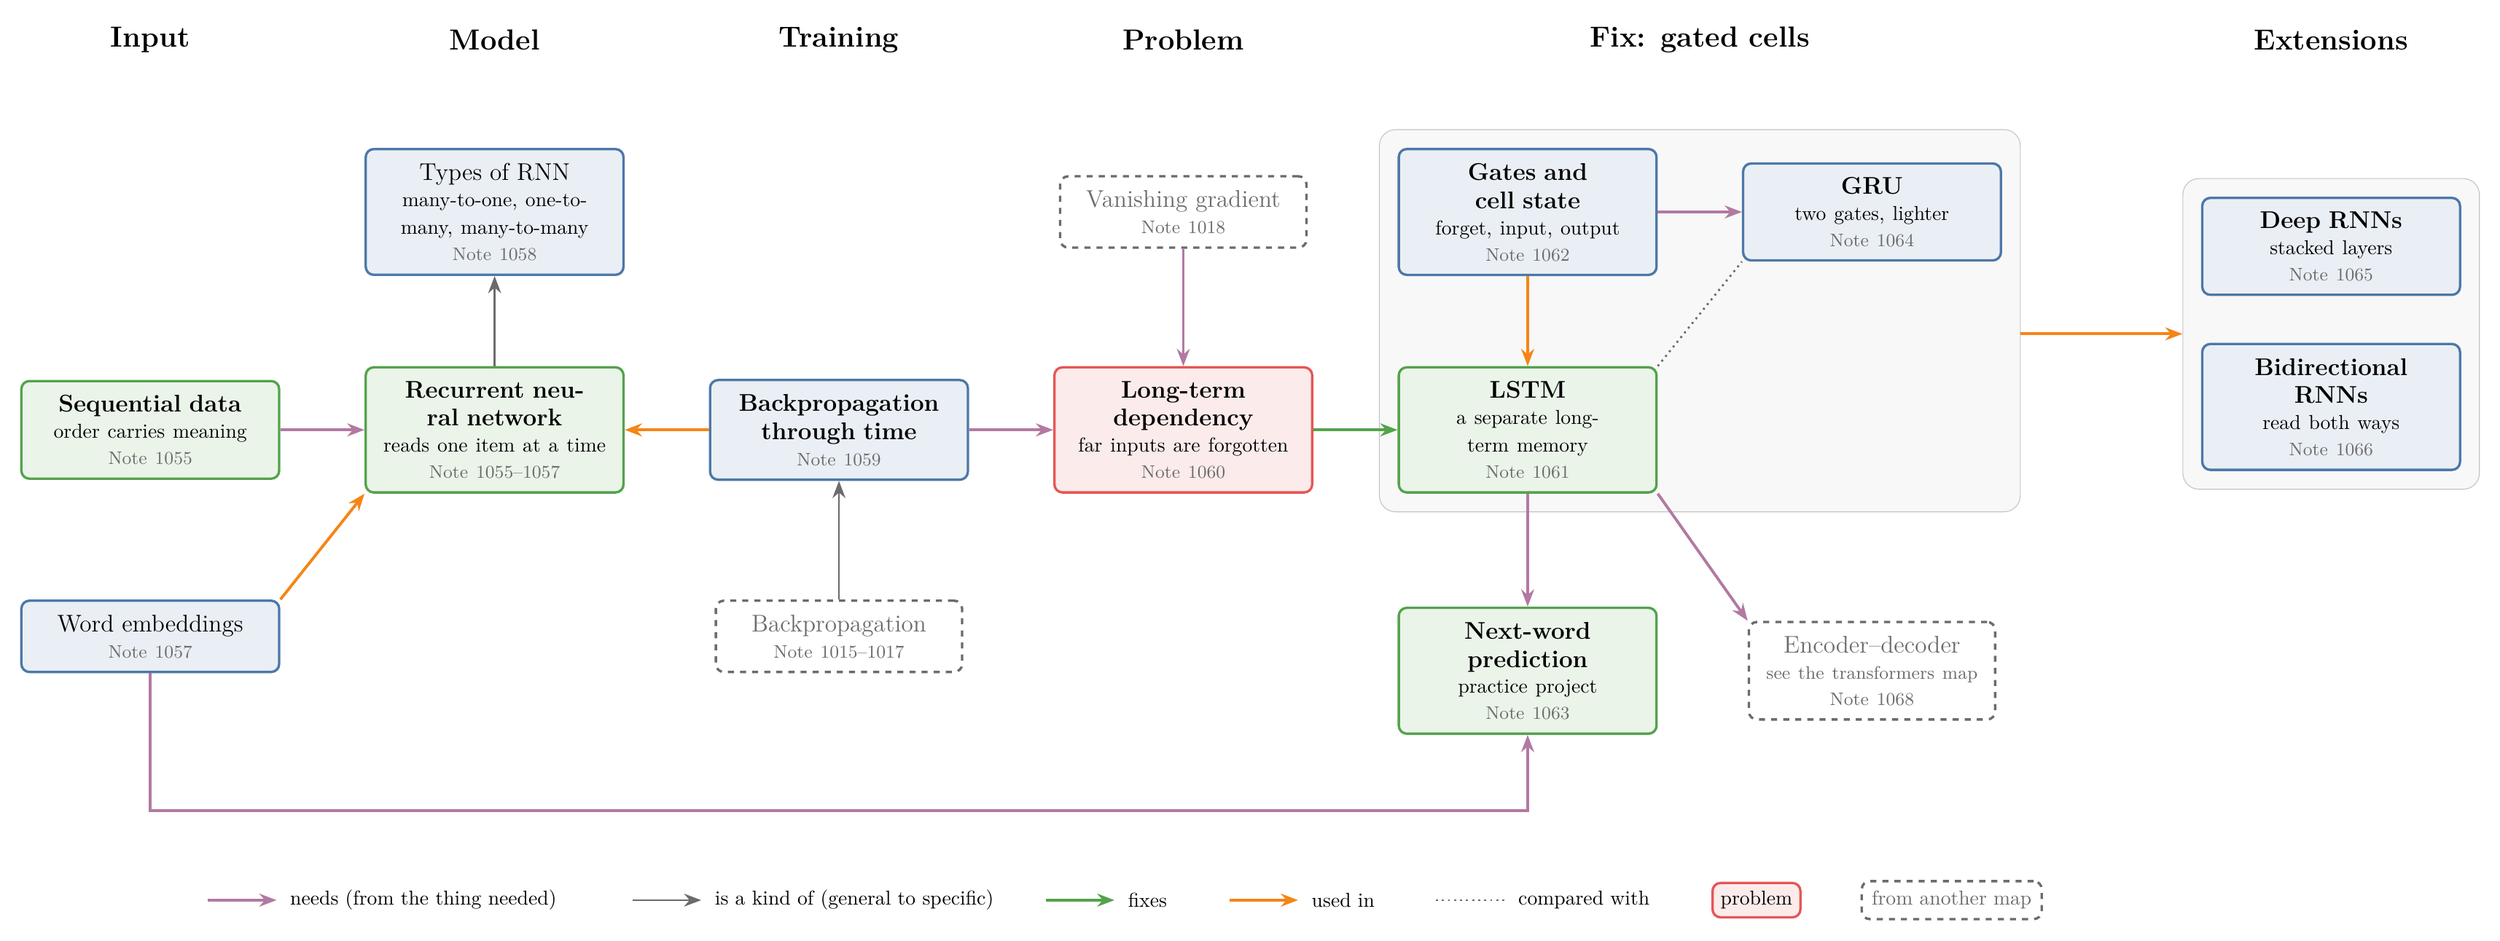
\begin{tikzpicture}[
    every node/.append style={font=\sffamily\large},
    con/.style={box=cblue, text width=4.0cm},
    prob/.style={box=cred, text width=4.0cm},
    prev/.style={draw=cgrey, dashed, rounded corners=4pt, align=center, inner sep=7pt, text=cgrey, text width=3.8cm, minimum height=1.1cm},
    group/.style={draw=cgrey!40, fill=cgrey!5, rounded corners=8pt, inner sep=9pt},
    kind/.style={arrow, draw=cgrey, line width=1pt},
    needs/.style={arrow, draw=cpurple},
    fixes/.style={arrow, draw=cgreen},
    usedin/.style={arrow, draw=corange},
    cmp/.style={draw=cgrey, line width=1pt, dotted},
  ]
  \newcommand{\nt}[1]{\\[-1pt]{\small\color{cgrey}Note #1}}
  \newcommand{\sub}[1]{\\[-1pt]{\normalsize #1}}
  \node[title] at (0,8.0) {Input};
  \node[title] at (6,8.0) {Model};
  \node[title] at (12,8.0) {Training};
  \node[title] at (18,8.0) {Problem};
  \node[title] at (27,8.0) {Fix: gated cells};
  \node[title] at (38,8.0) {Extensions};

  % input
  \node[box=cgreen, text width=4.0cm] (seq) at (0,1.2) {\textbf{Sequential data}\sub{order carries meaning}\nt{1055}};
  \node[con] (emb) at (0,-2.4) {Word embeddings\nt{1057}};

  % model
  \node[box=cgreen, text width=4.0cm, minimum height=2.0cm] (rnn) at (6,1.2) {\textbf{Recurrent neural network}\sub{reads one item at a time}\nt{1055--1057}};
  \node[con] (types) at (6,5.0) {Types of RNN\sub{many-to-one, one-to-many, many-to-many}\nt{1058}};
  \draw[needs] (seq) -- (rnn);
  \draw[usedin] (emb.north east) -- (rnn.south west);
  \draw[kind] (rnn) -- (types);

  % training
  \node[con] (bptt) at (12,1.2) {\textbf{Backpropagation through time}\nt{1059}};
  \node[prev] (bp) at (12,-2.4) {Backpropagation\nt{1015--1017}};
  \draw[usedin] (bptt) -- (rnn);
  \draw[kind] (bp) -- (bptt);

  % problem
  \node[prob] (ltd) at (18,1.2) {\textbf{Long-term dependency}\sub{far inputs are forgotten}\nt{1060}};
  \node[prev] (van) at (18,5.0) {Vanishing gradient\nt{1018}};
  \draw[needs] (bptt) -- (ltd);
  \draw[needs] (van) -- (ltd);

  % fix: gated cells
  \node[box=cgreen, text width=4.0cm, minimum height=2.0cm] (lstm) at (24,1.2) {\textbf{LSTM}\sub{a separate long-term memory}\nt{1061}};
  \node[con] (gates) at (24,5.0) {\textbf{Gates and cell state}\sub{forget, input, output}\nt{1062}};
  \node[con] (gru) at (30,5.0) {\textbf{GRU}\sub{two gates, lighter}\nt{1064}};
  \begin{scope}[on background layer]
    \node[group, fit=(lstm) (gates) (gru)] (gg) {};
  \end{scope}
  \draw[fixes] (ltd) -- (lstm);
  \draw[usedin] (gates) -- (lstm);
  \draw[needs] (gates) -- (gru);
  \draw[cmp] (lstm.north east) -- (gru.south west);

  % practice and next map
  \node[box=cgreen, text width=4.0cm] (nwp) at (24,-3.0) {\textbf{Next-word prediction}\sub{practice project}\nt{1063}};
  \node[prev] (s2s) at (30,-3.0) {Encoder--decoder\\[-1pt]{\small see the transformers map}\nt{1068}};
  \draw[needs] (lstm) -- (nwp);
  \draw[needs] (lstm.south east) -- (s2s.north west);
  \draw[needs] (emb.south) -- ++(0,-2.4) -| (nwp.south);

  % extensions
  \node[con] (deep) at (38,4.4) {\textbf{Deep RNNs}\sub{stacked layers}\nt{1065}};
  \node[con] (bi) at (38,1.6) {\textbf{Bidirectional RNNs}\sub{read both ways}\nt{1066}};
  \begin{scope}[on background layer]
    \node[group, fit=(deep) (bi)] (ge) {};
  \end{scope}
  \draw[usedin] (gg.east |- ge.center) -- (ge.west);

  % legend
  \begin{scope}[shift={(1.0,-7.0)}, every node/.style={font=\sffamily, anchor=west}]
    \draw[needs] (0,0) -- (1.2,0);      \node at (1.3,0) {needs (from the thing needed)};
    \draw[kind] (7.4,0) -- (8.6,0);     \node at (8.7,0) {is a kind of (general to specific)};
    \draw[fixes] (14.6,0) -- (15.8,0);  \node at (15.9,0) {fixes};
    \draw[usedin] (17.8,0) -- (19.0,0); \node at (19.1,0) {used in};
    \draw[cmp] (21.4,0) -- (22.6,0);    \node at (22.7,0) {compared with};
    \node[box=cred, minimum height=0.6cm, inner sep=4pt, anchor=west] at (26.2,0) {problem};
    \node[draw=cgrey, dashed, rounded corners=4pt, inner sep=5pt, text=cgrey, anchor=west] at (28.8,0) {from another map};
  \end{scope}
\end{tikzpicture}
\end{document}
